\documentclass[english,a4paper,pdftex]{report}
\usepackage[a4paper]{geometry}
\geometry{verbose,tmargin=1in,bmargin=1in,lmargin=1in,rmargin=1in}
\usepackage[pdftex]{graphicx}
\usepackage[backref,hidelinks = true]{hyperref}
\usepackage{natbib}

\begin{document}
%include the title
\begin{titlepage}
\title{{\Huge Report and Planning}}
\author{Willem Vaandrager 4175115 \\
\and Elgar de Groot 4091108 \\
\and Johnny Verhoeff 4137175 \\
\and Hugo Reinbergen 4161173 \\
\and Koos van der Linden 4133145}
\date{\today \\ Final version}
\maketitle
\end{titlepage}
\newpage

\begin{abstract}
The problem of Social Phobia in has been prevalent for a considerable time. A way to try and solve this problem is integrating an eCoach. The effect is even stronger when using an visual eCoach. The treatment with computer assistant makes patients more willing to keep participating in the program and will perform the activities more actively and with bigger steps.
\paragraph{}
 Treatment with an eCoach reduces travel time, it gives possibilities for a more comfortable environment, test results will be saved automatically and the workload of the therapists is reduced, which enables therapists to maintain more patients at the same time.
On the other hand, people feel less connected to a virtual avatar than an actual therapist, they require some form of computer knowledge and the eCoaches currently do not have high enough intelligence to completely replace a therapist.
\paragraph{}
To ensure a good result, the eCoach must be seen and heard, The avatar should be picked by the therapist, not the patient and the facial expression should be as close as possible to those from humans.

\end{abstract}

%make the table of contents
\tableofcontents

\chapter{Introduction}
The problem of Social Phobia in our society has been prevalent for a considerable time. A problem with curing this type of phobia is that in vivo treatment can be difficult: those exposure treatments most of the time require the presence of other people. A possible solution to this problem is virtual exposure, or maybe even better: virtual exposure at home.
\paragraph{}
But how do you motivate the patient at home to continue to attend the treatment? A solution could be to use an eCoach. An eCoach is a device or program that can be used by the therapist as a tool to act in behalf of the therapist when the patient is at home. Using an eCoach could create an easier environment for the patient to be treated in and could make the decision to ask for treatment easier and could speed up the process.
\paragraph{}
The question that remains is: what is the effect of the eCoach on the treatment of a patient with social phobia? This report will try to give an answer to this question. The expectation is that there will be some positive effect on the motivation of the major part of the users. This will probably result in a decrease of the avoidance and drop out of the treatment. Not all users will have benefit of the eCoach because of personal reasons.
\paragraph{}
To answer the main question some other questions need answering. The report will start off with how big the effect of the eCoach is on the motivation of the user (compared to conventional treatments). Next will be a description of the advantages of an eCoach, and of course also the disadvantages. Last will be some requirements for an eCoach system to achieve the effect mentioned.




\chapter{Influence on motivation}
The obvious benefit of home coaching is of course that the patient doesn't have to leave his home. Virtual coaches exist in many different forms: as a mobile running application that tells you when it's time to go for another run, or as an annoying paper-clip that asks you what you want to do in a text editor.  The effectiveness of a virtual coach has been proven in different fields. One study found that beginning athletes did more exercising with a virtual coach than without \cite{eyck2006effect}. 
\paragraph{}
But how much influence has a visual representation of an eCoach on the behaviour of people (patients)? In a study \cite{rosenberg2007importance} where young women are motivated towards engineering, the study group found that a visual presence of an eCoach had significantly more influence on the women than with a voice-only coach. This is very interesting, because it not only proves that a visual coach helps, but is even better than a non-visual eCoach. When the coach can be seen and not only heard, people have more the perception they are really interacting with someone \cite{baylor2009promoting}. 
\paragraph{}
It seems that an eCoach can have a significant effect on a person that interacts with it, so if the effect is as strong with social phobic persons, an eCoach would be a promising tool to motivate them in continuing their treatment.



\chapter{Advantages of eCoaching}
\begin{itemize}
\item Patients don't have to travel to another city, possibly during rush hour, because they can just do the therapy at home.
\item The environment, in which the patients are exposed, can be manipulated in every way, whereas real life with real human beings can't. 
Some manipulations:
	\begin{itemize}
	\item Gender, age, ethnicity.
	\item Quantity of avatars in the environment.
	\item Responses of every avatar can be controlled.
	\end{itemize}
\item The eCoach isn't a replacement for the actual therapist; it is only a form of treatment, which is still guided by a real therapist, doing it from the convenience of his own home.
\item All progress that a patients makes and all parameters that can be measured from a patient, such as SUD scores, will be automatically saved and send to a database. So the therapist doesn't have to do it himself and he/she can have access to it anywhere and any time in the form of diagrams and/or graphs.
\item The eCoach can also talk outside the exposure to the patient, about what the patient experiences outside the sessions in real life for example. Now the therapist also does, but most of the time the therapist feigns interest, he/she only does it as a courtesy to the patient.
\item Because the therapist doesn't need to do everything by himself during an exposure, it reduces the workload of a therapist. Now the therapist has more time to closely monitor the patient's progress and can adjust treatment accordingly.  Also he is able to deal with more patients because of the time benefit.\cite{ter2011design}
\end{itemize}



\chapter{Disadvantages of eCoaching}
eCoaching contains a lot of advantages with helping patients, but there are also some disadvantages we should consider. 
\paragraph{}
People feel less connected to an avatar or robot than a human and will feel less emotional letting down an avatar \cite{clutterbuck2009virtual}. A disadvantage that follows from this is reduced commitment. It is easier to abandon a task an avatar assigned than one assigned by the therapist. They feel there will be less consequences and will sooner disengage from eCoaches.
\paragraph{}
A long with the commitment issue, eCoaches are also harder to use for some people. Not everyone is familiar with using computers and might not be able to use the eCoach fully as they were intended to use. It is possible they cannot get the program to work or do not know how to work with the program. Interacting with an avatar can feel unnatural to some people as well. These problems may ensure that the therapy is not working optimally or at all and will slow down the progress to get over their social phobia.
\paragraph{}
eCoaches are not as good as people, yet. The avatars might end up in a situation they cannot handle and can provide strange answers, which have nothing to do with the conversation and can confuse the patient by doing so. 
\paragraph{}
A simulated world with avatars will also be less realistic than the real world. Patients trained solely in the simulated world might be adapted to the avatars and are still not able to handle certain situations in the real world. They can also still get scared from actual person instead of avatars, because they feel it more real and are still not comfortable with handling with actual persons.  


\chapter{Difference with regular treatment}
A problem with traditional eHealthcare and self-management is that patients lose motivation over time. They begin with good will since they've just decided to start fighting their anxiety. The decision to start treatment is rather heavy, so once the choice is made to start treatment, the patients are motivated to do their absolute best to change their selves. But it is shown \cite{alpay2007} that this motivation slowly degenerates as the treatment progresses. Patients fill in the forms required for the treatment less often and stop the treatment altogether. The same study says that physical interventions during the treatment period refreshed the motivation.
\paragraph{}
Physical interventions bring their own trouble with them since they require people to actively involve themselves with others. But an eCoach can fill in the same role. With an eCoach, or Computer Assistant, the patients stay more motivated over the duration of the treatment. This is illustrated in the image below, which is taken from a study on the effects of a computer assistant on a plan for weight loss \cite{blanson2009online}.\\
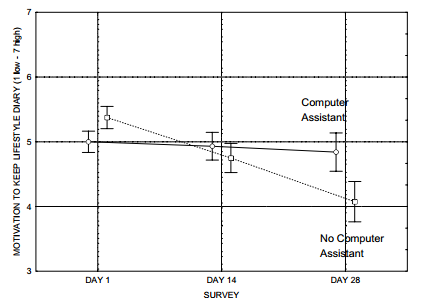
\includegraphics[scale=0.8]{Graph1.png}
\paragraph{}
Other than the patients being more active with filling in the results of their treatment, the same study shows that the patients also are more willing to actively achieve the goals set for them, when an eCoach is supporting and motivating them. This is illustrated below.\\
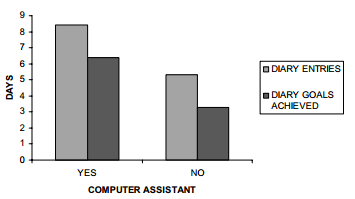
\includegraphics[scale=1]{Graph2.png}
\paragraph{}
These results show that there is a significant difference in the motivation levels of patients during treatment with an eCoach and without. This is especially noticeable in the later stages of the program.


\chapter{Criteria for success}
So far it has been pointed out that virtual exposure at home is at least as effective as in vivo treatment. But what is needed to achieve this result? Different properties will be discussed here. First the visibility of the avatar will be discussed. Secondly the appearance of the avatar will be discussed, and finally the contribution of the facial expressions of the avatar.
\paragraph{}
The avatar that interacts with the patient as an eCoach must not only be heard, but also seen \cite{baylor2009promoting}. It can enhance the idea that the eCoach is actually present in the same room. Whether the avatar was static or dynamic didn't really seem to matter, but being visible did.
\paragraph{}
The appearance of this visible avatar also matters. Different test have been done with groups that were allowed to choose their own coaching avatar, and others that were appointed an avatar based on professional analysis \cite{baylor2009promoting}. Most of the time patients didn't choose the avatar that suited them best, so it better not to let the patient choose the avatar for his/her coach. It would be good though to let the therapist choose an appropriate avatar.
\paragraph{}
Also the use of facial expressions contributes to the effect of the eCoach. The visible emotions (such as sad or neutral) enhance the idea of empathy of the avatar \cite{blanson2009online} and hence will increase the anthropomorphic experience of the avatar.


\chapter{Conclusion}
We saw that an eCoach can have a significant positive influence on the motivation of patients to continue with treatment. This effect is even greater with a visual eCoach. On top of that it has a number of advantages over regular coaching, such as workload reduction for the therapist and more exposure time for the patient.
\paragraph{}
There are some drawbacks to an eCoach. People still feel less connected to a virtual coach than to an actual coach, the eCoach might not be able to handle all situations and some people have difficulties using a computer.
\paragraph{}
However, when comparing regular treatment to treatment with an eCoach, the eCoach has the upper hand and results in more consistent motivation. In conclusion, our hypothesis seems to hold and there is a positive effect on the motivation of the major part of the users. There are some things that have influence on the success of the eCoach, such as the appearance of the avatar and the emotions it shows. These have to be considered when working with a visual eCoach.



%include the references
\bibliographystyle{plain}
\bibliography{references}

\end{document}